\documentclass[10pt]{article}
\usepackage[utf8]{inputenc}
\usepackage[T1]{fontenc}
\usepackage{amsmath}
\usepackage{amsfonts}
\usepackage{amssymb}
\usepackage[version=4]{mhchem}
\usepackage{stmaryrd}
\usepackage{graphicx}
\usepackage[export]{adjustbox}
\graphicspath{ {./images/} }

\begin{document}

    The Event Horizon Telescope (EHT) has released an image of the supermassive black hole at the centre of the M87 galaxy as shown in the left panel of the figure below.

    To understand some simple features of this image, we will consider a simplified model of a non-rotating, static, spherically symmetric black hole of mass $M=6.5 \times 10^{9} \mathrm{M}_{\odot}$, surrounded by a massless, thin, planar accretion disk of inner and outer radii, $a_{\text {inner }}=6 R_{\text {SC }}$ and $a_{\text {outer }}=10 R_{\text {SC }}$, respectively, where $R_{\text {SC }}$ is the Schwarzschild radius. A face-on view sketch is shown in the right panel of the figure below (figure is not to scale).\\
    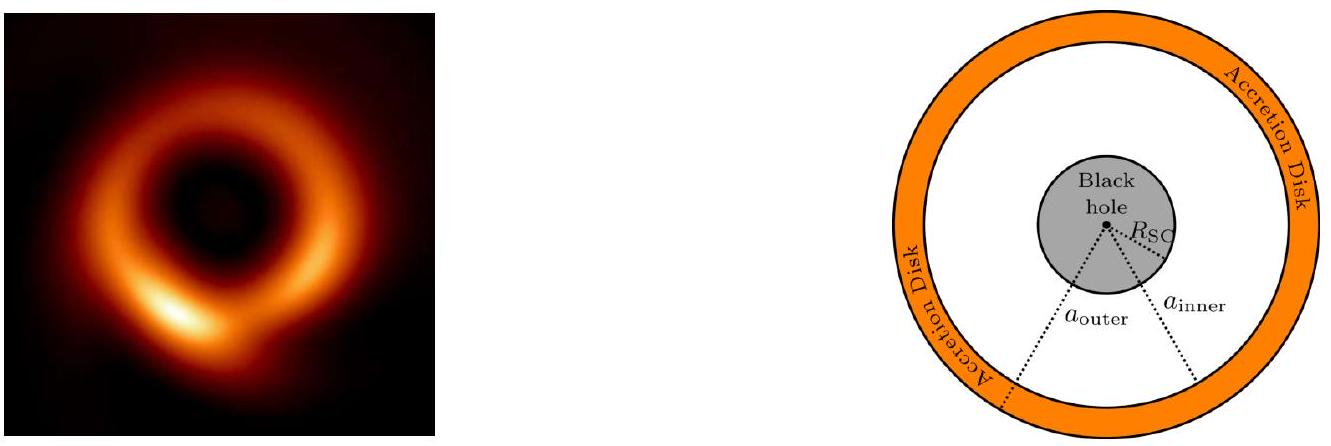
\includegraphics[max width=\textwidth, center]{2025_08_23_e94579452776a99c4850g-07}
    
    We assume that the accretion disk is the only source of light to be considered. Every point on the disk emits light in all directions. This light travels under the influence of the gravitational field of the black hole. The path of the light rays is governed by two equations given below (which are similar to those of an object around the Sun):
    
    $$
    \frac{1}{2} v_{\mathrm{r}}^{2}+\frac{L^{2}}{2 r^{2}}\left(1-\frac{2 G M}{c^{2} r}\right)=E \quad ; \quad v_{\phi}=r \omega=\frac{L}{r}
    $$
    
    where $r \in\left(R_{\mathrm{SC}}, \infty\right)$ is the radial coordinate, $\phi \in[0,2 \pi)$ is the azimuthal angle, and $E$ and $L$ are constants related to the conserved energy and conserved angular momentum, respectively.
    
    Here $v_{\mathrm{r}} \equiv d r / d t$ is the magnitude of the radial velocity, $v_{\phi}$ is the magnitude of the tangential velocity, and $\omega \equiv d \phi / d t$ is the angular velocity. We define the impact parameter $b$ for a trajectory as $b=L / \sqrt{2 E}$. Time dilation is neglected in this problem.
    
    Another useful equation is obtained by differentiating the first equation:
    
    $$
    \frac{d v_{\mathrm{r}}}{d t}-\frac{L^{2}}{r^{3}}+\frac{3 G M L^{2}}{c^{2} r^{4}}=0
    $$
    
    (T08.1) Circular light trajectories can exist around the black hole. Find the radius, $r_{\mathrm{ph}}$, and impact parameter, $b_{\mathrm{ph}}$, for such photon trajectories in terms of $M$ and relevant constants.\\
    (T08.2) Calculate the time, $T_{\mathrm{ph}}$, taken for completing one full orbit of the circular light trajectory in seconds.\\
    (T08.3) The radial velocity equation given above (the first equation in this question) can be compared with an equation of the form $\frac{v_{\mathrm{r}}^{2}}{2}+V_{\text {eff }}(r)=E$ for light trajectories. A schematic plot of $V_{\text {eff }} / L^{2}$ as a function of $r$ is given below.\\
    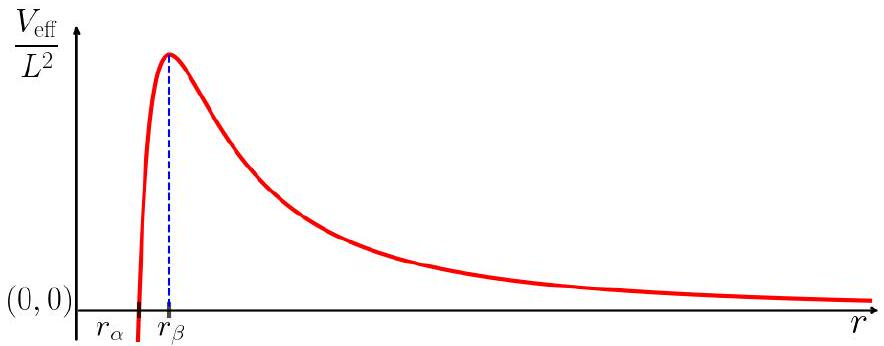
\includegraphics[max width=\textwidth, center]{2025_08_23_e94579452776a99c4850g-08}\\
    (T08.3a) The plot indicates two special radii, $r_{\alpha}$ and $r_{\beta}$. Obtain expressions for $r_{\alpha}$ and $r_{\beta}$ in terms of $M$ and relevant constants.\\
    (T08.3b) A photon travelling inward from the accretion disk towards the black hole can still escape out to infinity in some cases. Find the expression for the smallest value of the turning point radius, $r_{\mathrm{t}}$, for such a photon, in terms of $M$ and relevant constants. Find the expression for the minimum value of the impact parameter, $b_{\text {min }}$, for this photon.\\
    (T08.4) A ray of light coming from a radius $r_{\text {actual }}$ from the centre of the system in the plane of the sky will suffer strong bending due to the gravity of the black hole, and eventually reach an observer (denoted by an eye) at a large distance $d$ from the system, as shown below.\\
    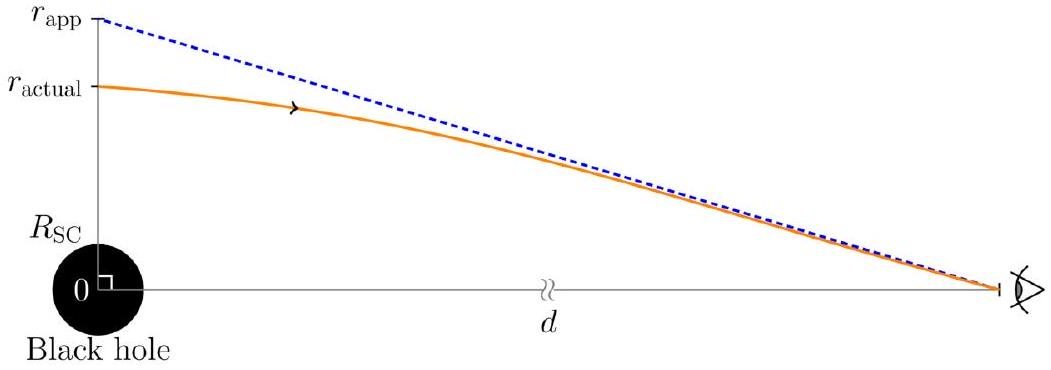
\includegraphics[max width=\textwidth, center]{2025_08_23_e94579452776a99c4850g-08(1)}
    
    To this observer, the ray would appear to have originated from a different point at a distance $r_{\text {app }} \approx b$ from the black hole centre in the plane of the sky, where $b$ is the impact parameter for that photon trajectory. For points on the accretion disk at $r=r_{\text {actual }}$, one may assume the following relation:
    
    $$
    b\left(r_{\text {actual }}\right) \approx r_{\text {actual }}\left(1+R_{\mathrm{SC}} / r_{\text {actual }}\right)^{1 / 2}
    $$
    
    For the distant observer, like ourselves, with a face-on view of the accretion disk, the image of the system will appear to be circularly symmetric in the plane of the sky. Determine the outermost apparent radius, $r_{\text {outer }}$, and the innermost apparent radius, $r_{\text {inner }}$, of the image in units of au.\\
    (T08.5) Consider an isolated supermassive black hole of mass $M=6.5 \times 10^{9} \mathrm{M}_{\odot}$ without any accretion disk. A brief strong burst of electromagnetic radiation occurs for 5 s at a point Z at a distance, say, $r_{\mathrm{Z}}=6 R_{\mathrm{SC}}$ from the black hole as shown in the figure. The burst at point Z emits light in all directions. An observer at a point far from the black hole (denoted by an eye in the figure below) takes a long exposure image of the region around the black hole for 60 s .\\
    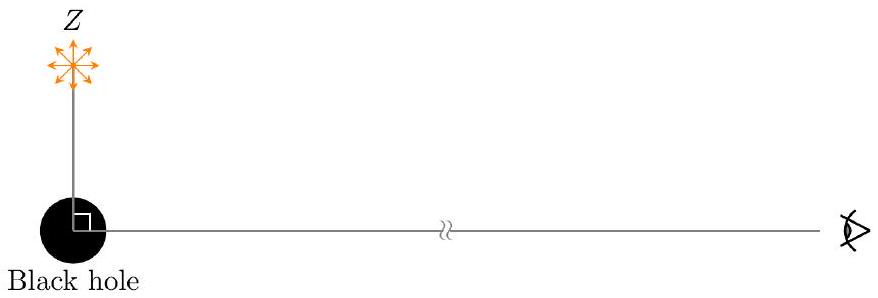
\includegraphics[max width=\textwidth, center]{2025_08_23_e94579452776a99c4850g-09}
    
    Choose the correct option for each of the statements below:\\
    (T08.5a) The number of possible paths for light to travel from Z to the observer is (A) At most one (B) Exactly one (C) Exactly two (D) Greater than two.\\
    (T08.5b) The number of images of the EM burst at Z that will be seen in the long exposure image is (A) At most one (B) Exactly one (C) Exactly two (D) Greater than two.\\

\end{document}